\documentclass[11pt]{article}
\usepackage[utf8]{inputenc}
\usepackage[T1]{fontenc}
\usepackage{amsmath}
\usepackage{amssymb}
\usepackage{multicol}
\usepackage{geometry}
\usepackage{tikz}
\usepackage{enumitem}
\usepackage{xcolor}
\usepackage{titlesec}

% Configurações de layout
\geometry{a4paper, left=1cm, right=1cm, top=0.5cm, bottom=1.2cm}
\setlength{\columnseprule}{0.4pt}

% Cores para títulos
\titleformat{\section}{\normalfont\Large\bfseries\color{blue}}{\thesection}{1em}{}
\titleformat{\subsection}{\normalfont\large\bfseries\color{red}}{\thesubsection}{1em}{}

\title{\textcolor{red}{Primeiro Trimestre: Funções
    \\Função do Primeiro Grau}}
\author{Professor: Jefferson}
\date{}

\begin{document}

\maketitle
\vspace{-1cm}

%\begin{center}
%\large{Nome: \underline{\hspace{8cm}} \quad Turma: \underline{\hspace{3cm}}}
%\end{center}

\begin{multicols}{2}

\section*{Conceitos Básicos}

\subsection*{Função}
Relação entre dois conjuntos onde cada elemento do primeiro conjunto (domínio) corresponde a exatamente um elemento do segundo conjunto (contradomínio).

\subsection*{Função do Primeiro Grau (Afim)}
Função que pode ser escrita na forma:
\[
f(x) = ax + b
\]
onde $a \neq 0$.

\subsection*{Variáveis}
\begin{itemize}
\item $a$: coeficiente angular (inclinação da reta)
\item $b$: coeficiente linear (intercepto no eixo $y$)
\item $x$: variável independente
\item $f(x)$ ou $y$: variável dependente
\end{itemize}

\subsection*{Características}
\begin{itemize}
\item \textbf{Domínio}: geralmente $\mathbb{R}$
\item \textbf{Imagem}: geralmente $\mathbb{R}$
\item \textbf{Crescimento linear} (progressão aritmética)
\item \textbf{Gráfico}: uma reta
\item \textbf{Biunívoca}: cada $y$ corresponde a um único $x$
\end{itemize}

\section*{Classificação das Funções do 1º Grau}

\subsection*{Função Crescente}
Quando $a > 0$, a função é crescente.

Exemplo: $f(x) = 2x + 3$

\subsection*{Função Decrescente}
Quando $a < 0$, a função é decrescente.

Exemplo: $f(x) = -3x + 5$

\subsection*{Função Linear}
Quando $b = 0$, a função é linear.

Exemplo: $f(x) = 2x$

\section*{Raiz (Zero) da Função}

A raiz é o valor de $x$ onde $f(x) = 0$:

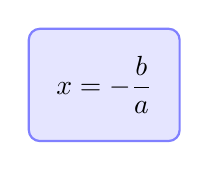
\begin{tikzpicture}
\node[rectangle, fill=blue!10, rounded corners, inner sep=10pt, draw=blue!50, thick] (box) {
$\displaystyle x = -\frac{b}{a}$
};
\end{tikzpicture}

\subsection*{Interpretação Geométrica}
A raiz é o ponto onde a reta cruza o eixo $x$.

\section*{Pontos Importantes da Função}

\subsection*{Intercepto no Eixo Y}
Ponto $(0, b)$ - onde a reta cruza o eixo $y$.

Obtém-se fazendo $x = 0$:
\[
f(0) = a(0) + b = b
\]

\subsection*{Intercepto no Eixo X}
Ponto $\left(-\frac{b}{a}, 0\right)$ - onde a reta cruza o eixo $x$.

Obtém-se fazendo $f(x) = 0$.

\section*{Representação Gráfica}

\begin{center}
\begin{tikzpicture}[scale=0.8]
\draw[->] (-1,0) -- (4,0) node[right] {$x$};
\draw[->] (0,-1) -- (0,4) node[above] {$y$};
\draw[blue, thick, domain=-0.5:3.5] plot (\x, {0.5*\x + 1}) node[right] {$f(x) = 0,5x + 1$};
\draw[dashed] (0,1) -- (-0.2,1) node[left] {$b$};
\draw[dashed] (-2,0) -- (-2,-0.2) node[below] {$-b/a$};
\fill[blue] (0,1) circle (2pt) node[above right] {$(0, b)$};
\fill[blue] (-2,0) circle (2pt) node[below left] {Raiz};
\end{tikzpicture}
\end{center}

\section*{Exercícios Básicos - Função do 1º Grau}

\begin{enumerate}[leftmargin=*]

\item Identifique o coeficiente angular e linear:
\begin{enumerate}[label=\alph*)]
\item $f(x) = 2x + 5$
\item $f(x) = -3x + 1$
\item $f(x) = 4x$
\item $f(x) = -x + 2$
\end{enumerate}

\item Calcule $f(x)$ para os valores dados:
\begin{enumerate}[label=\alph*)]
\item $f(x) = 3x + 2$ para $x = 0, 1, 2, 3$
\item $f(x) = -2x + 5$ para $x = -1, 0, 1, 2$
\item $f(x) = 5x$ para $x = 2, 4, 6$
\end{enumerate}

\item Encontre a raiz (zero) da função:
\begin{enumerate}[label=\alph*)]
\item $f(x) = 2x - 6$
\item $f(x) = -3x + 9$
\item $f(x) = 4x + 8$
\item $f(x) = -5x + 10$
\end{enumerate}

\item Classifique em crescente ou decrescente:
\begin{enumerate}[label=\alph*)]
\item $f(x) = 3x + 1$
\item $f(x) = -2x + 4$
\item $f(x) = 5x - 3$
\item $f(x) = -4x + 7$
\end{enumerate}

\end{enumerate}

\section*{Forma Ponto-Coeficiente Angular}

\subsection*{Fórmula}
Se conhecemos um ponto $(x_1, y_1)$ e o coeficiente angular $a$:

\[
y - y_1 = a(x - x_1)
\]

Ou equivalentemente:
\[
y = a(x - x_1) + y_1
\]

\subsection*{Exemplo}
Determinar a função que passa por $(2, 5)$ com $a = 3$:
\[
y - 5 = 3(x - 2)
\]
\[
y = 3x - 6 + 5 = 3x - 1
\]

\section*{Forma Dois Pontos}

\subsection*{Fórmula}
Se conhecemos dois pontos $(x_1, y_1)$ e $(x_2, y_2)$:

\[
a = \frac{y_2 - y_1}{x_2 - x_1}
\]

Depois use a forma ponto-coeficiente angular.

\subsection*{Exemplo}
Pontos $(1, 3)$ e $(3, 7)$:
\[
a = \frac{7 - 3}{3 - 1} = \frac{4}{2} = 2
\]
\[
y - 3 = 2(x - 1) \Rightarrow y = 2x + 1
\]

\section*{Exercícios Intermediários}

\begin{enumerate}[leftmargin=*, start=5]

\item Determine a função que passa por:
\begin{enumerate}[label=\alph*)]
\item Ponto $(1, 3)$ com $a = 2$
\item Ponto $(0, 4)$ com $a = -1$
\item Ponto $(2, 1)$ com $a = 3$
\end{enumerate}

\item Determine a função dados dois pontos:
\begin{enumerate}[label=\alph*)]
\item Pontos $(1, 2)$ e $(3, 8)$
\item Pontos $(0, 5)$ e $(2, 1)$
\item Pontos $(1, 1)$ e $(4, 4)$
\end{enumerate}

\item Análise completa de funções:
\begin{enumerate}[label=\alph*)]
\item $f(x) = 2x - 4$: encontre raiz, $f(0)$, $f(3)$
\item $f(x) = -3x + 6$: encontre raiz, $f(0)$, $f(1)$
\end{enumerate}

\item Problemas contextualizados:
\begin{enumerate}[label=\alph*)]
\item A temperatura em graus Celsius é $T(t) = 20 + 5t$, onde $t$ é o tempo em horas. Qual a temperatura inicial e após 3 horas?
\item O custo de produção é $C(x) = 50 + 10x$, onde $x$ é a quantidade produzida. Qual o custo inicial e para 50 unidades?
\item A altura de uma árvore é $h(t) = 1,5 + 0,3t$, onde $t$ é em anos. Qual a altura inicial e após 10 anos?
\end{enumerate}

\end{enumerate}

\section*{Sinal da Função}

Para $f(x) = ax + b$:

\subsection*{Quando $a > 0$ (Crescente)}
\begin{itemize}
\item $f(x) > 0$ quando $x > -\frac{b}{a}$
\item $f(x) = 0$ quando $x = -\frac{b}{a}$
\item $f(x) < 0$ quando $x < -\frac{b}{a}$
\end{itemize}

\subsection*{Quando $a < 0$ (Decrescente)}
\begin{itemize}
\item $f(x) < 0$ quando $x > -\frac{b}{a}$
\item $f(x) = 0$ quando $x = -\frac{b}{a}$
\item $f(x) > 0$ quando $x < -\frac{b}{a}$
\end{itemize}

\section*{Exercícios Avançados}

\begin{enumerate}[leftmargin=*, start=8]

\item Estude o sinal das funções:
\begin{enumerate}[label=\alph*)]
\item $f(x) = 2x - 4$
\item $f(x) = -3x + 6$
\item $f(x) = 5x + 10$
\end{enumerate}

\item Função inversa:
\begin{enumerate}[label=\alph*)]
\item Encontre a inversa de $f(x) = 2x + 3$
\item Encontre a inversa de $f(x) = -x + 5$
\item Verifique: $f(f^{-1}(x)) = x$
\end{enumerate}

\item Composição de funções:
\begin{enumerate}[label=\alph*)]
\item $f(x) = 2x + 1$ e $g(x) = 3x - 2$. Calcule $f(g(x))$ e $g(f(x))$
\item $f(x) = x + 5$ e $g(x) = 2x$. Calcule $f(g(2))$ e $g(f(3))$
\end{enumerate}

\item Sistemas de equações com funções do 1º grau:
\begin{enumerate}[label=\alph*)]
\item Encontre o ponto de interseção de $f(x) = 2x + 1$ e $g(x) = -x + 4$
\item Encontre o ponto de interseção de $f(x) = 3x - 2$ e $g(x) = x + 2$
\end{enumerate}

\end{enumerate}

\section*{Dicas Importantes}

\begin{itemize}
\item \textbf{Sempre} verifique o sinal do coeficiente angular para determinar crescimento
\item \textbf{A raiz} é o ponto onde a função cruza o eixo $x$
\item \textbf{O intercepto} $y$ é o valor de $b$
\item \textbf{Dois pontos} definem uma reta única
\item \textbf{Função linear} passa pela origem $(0, 0)$
\item \textbf{Use gráficos} para visualizar e verificar resultados
\end{itemize}

\end{multicols}

\end{document}
